\def\firstname{Tim}
\def\lastname{Dahmen}
\def\aufgabenblatt{5}

\documentclass{article}

\usepackage[a4paper, margin=2.5cm]{geometry}
\usepackage{graphicx}
\usepackage[ngerman]{babel} % automatische Silbentrennung
\usepackage[table]{xcolor}
\usepackage{tabularx,array,booktabs,makecell}
\usepackage{titlesec}
\usepackage{amsmath}

\usepackage{fancyhdr}
\pagestyle{fancy} 
\fancyhead[L]{Inpainting SS 2024}  

\fancypagestyle{page1}{
	\fancyhead[L]{\firstname \: \lastname}
	\fancyhead[C]{Inpainting SS 2024\\Aufgabenblatt \aufgabenblatt}
	\fancyhead[R]{ \\
\includegraphics[width=0.25\textwidth]{../common/hs_aalen_de.png}}

}
\setlength{\parindent}{0mm}
\setlength{\parskip}{2.5mm}

\titlespacing*{\section}{0mm}{4pt}{0pt}
\setlength{\headsep}{14mm}

\begin{document}
\thispagestyle{page1} 

\section{Patchbasiertes Inpainting mit Criminisi-Dataterm}

In dieser Aufgabe erweitern Sie das Inpainting (siehe Musterlösung oder Ihre eigene Implementierung) um den Dataterm gem. Criminisi et. al. 	

\begin{enumerate}

\item[a)] Lesen und verstehen Sie den relevanten Teil des Papers von Criminisi. \\ \texttt{https://www.irisa.fr/vista/Papers/2004\_ip\_criminisi.pdf}

\item[b)] Argumentieren Sie: wie könnte das Verfahren getested werden? Welche Schwierigkeit stellt sich für Unittests?

\item[c)] Erweitern Sie die Berechnung der Priorität auf der Fillfront um den Data Term.

\end{enumerate}

\section{k-Nearest Neighbor bestimmen}

In dieser Aufgabe implementieren Sie verschiedene Verfahren, um die k nächsten definiertem Nachbarn eines Pixels zu bestimmen. 

\subsection{Unit-Tests}

\begin{enumerate}

\item[a)] Implementieren Sie Unittests für das Verfahren.

\item[b)] Beschreiben Sie Ihre Teststrategie: welche Fälle testen Sie, und warum? Welche Rolle spielen Visualisierungen?

\end{enumerate}

Für die Bearbeitung der Aufgabe habe ich folgende Zeit benötigt:

\subsection{knn Bestimmung auf Pixelebene}

In dieser Aufgabe bestimmen Sie die k nächsten Nachbarn auf Pixelebene. In der Datei \texttt{knn\_search.ipynb} wurde bereits eine
brute-force-lösung implementiert. 

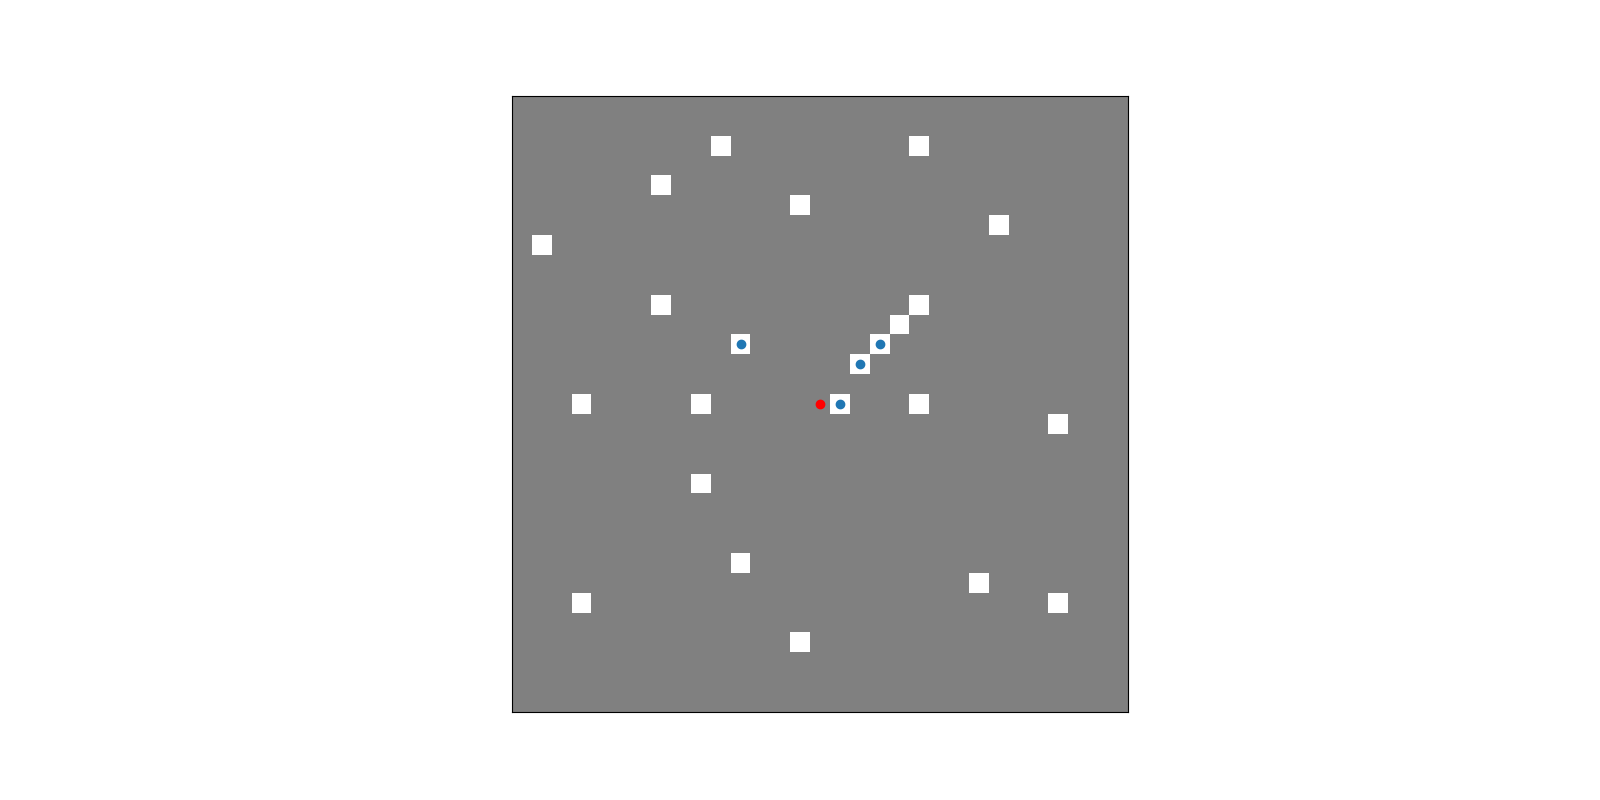
\includegraphics[width=0.75\textwidth]{source_code/knn_search_brute_force.png}

\begin{enumerate}

\item[a)] Implementieren Sie ein Verfahen, dass mittels Auflistung der Pixel (quadratische Auflistung) die k nächsten Nachbarn bestimmt.

\item[b)] Implementieren Sie ein Verfahen, dass mittels Auflistung der Pixel (zirkuläre Auflistung) die k nächsten Nachbarn bestimmt.

\end{enumerate}

Für die Bearbeitung der Aufgabe habe ich folgende Zeit benötigt:

\subsection{knn Bestimmung auf Graphebene}

\begin{enumerate}

\item[a)] Implementieren Sie nun ein Verfahen, dass die k nächsten Nachbarn auf Basis einer Delauney-Triangulierung bestimmt. Sie können die Klasse scipy.spatial.Delaunay nutzen.

\end{enumerate}

Für die Bearbeitung der Aufgabe habe ich folgende Zeit benötigt:

\subsection{Performance Vergleich}

\begin{enumerate}

\item[a)] Implementieren Sie nun einen Tests, der einen Performance Verleich der drei Verfahren erlaubt. Argumentieren Sie: wie müssen die Testfälle hinsichtlich Bildgröße,  Pixeldichte und Pixelverteilung aufgabaut sein? Profilen Sie alle drei Verfahren mit Hilfe des Python line profilers. 

\item[b)] Beschreiben Sie das Optimierungspotential aller drei Verfahren. Wählen Sie eines für weitere Optimierungen aus und begründen Sie die Entscheidung.

\end{enumerate}

Für die Bearbeitung der Aufgabe habe ich folgende Zeit benötigt:

\subsection{Performance Optimierung}

\begin{enumerate}

\item[a)] Optimieren Sie das ausgewählte Verfahren. 

\item[b)] Bewerten Sie die Ergebnisse Ihrer Optimierung. 

\end{enumerate}

Für die Bearbeitung der Aufgabe habe ich folgende Zeit benötigt:

\end{document}